  
\chapter{Verification Dataset}
\label{chapter:vds}

\section{Overview}

\begin{table}
\caption{ \smr\ VDS content for the various frequency modes of \smr\..}
\label{table:comp}
\scalebox{0.9}{%
\begin{tabular}{|l|l|l|l|l|}
\hline
\textbf{\smr}           & \textbf{\smr}            & \textbf{Instrument} &  \textbf{Species}                         & \textbf{Number of}\\
\textbf{Frequency mode} & \textbf{Frequency range [GHz]} &               &                                           & \textbf{measurements}\\     
\hline
                     01 &  501.180--501.580,       & SMILES              & \chem{O_3}, \chem{ClO}                    &   2398,1384  \\
                        &  501.980--502.380        & MLS                 & \chem{O_3}, \chem{ClO}, \chem{N_{2}O}     &  11050       \\
                        &                          & MIPAS               & \chem{O_3}, \chem{N_{2}O}                 &   7228       \\
                        &                          & SAGEIII             & \chem{O_3}                                &   3115       \\
\hline
                     02 &  544.102--544.902        & SMILES              & \chem{O_3}, \chem{HNO_3}                  &   2367,1353  \\
                        &                          & MLS                 & \chem{O_3}, \chem{HNO_3}                  &  10824       \\
                        &                          & MIPAS               & \chem{O_3}, \chem{HNO_3}                  &   7176       \\
                        &                          & SAGEIII             & \chem{O_3}                                &   3063       \\
\hline
                     08 &  488.950--489.350,       & SMILES              & \chem{O_3}                                &    618       \\
                        &  488.350--488.750        & MLS                 & \chem{O_3}, \chem{H_{2}O}                 &  10759       \\
                        &                          & MIPAS               & \chem{O_3}, \chem{H_{2}O}                 &   6249       \\
                        &                          & SAGEIII             & \chem{O_3}, \chem{H_{2}O}                 &    284       \\
\hline
                     13 &  556.598--557.398        & SMILES              & \chem{O_3}                                &    364       \\
                        &                          & MLS                 & \chem{O_3}, \chem{H_{2}O}                 &   9352       \\
                        &                          & MIPAS               & \chem{O_3}, \chem{H_{2}O}                 &   5001       \\
                        &                          & SAGEIII             & \chem{O_3}, \chem{H_{2}O}                 &    170       \\
\hline
                     14 &  576.062--576.862        & SMILES              & \chem{O_3}                                &    409       \\
                        &                          & MLS                 & \chem{O_3}, \chem{CO}                     &   9547       \\
                        &                          & MIPAS               & \chem{O_3}, \chem{CO}                     &   5005       \\
                        &                          & SAGEIII             & \chem{O_3}                                &    170       \\
\hline
                     17 &   489.950--490.750       & SMILES              & \chem{O_3}                                &    527       \\
                        &                          & MLS                 & \chem{O_3}, \chem{H_{2}O}                 &  10566       \\
                        &                          & MIPAS               & \chem{O_3}, \chem{H_{2}O}                 &   6126       \\
                        &                          & SAGEIII             & \chem{O_3}, \chem{H_{2}O}                 &    263       \\
\hline
                     19 &   556.550--557.350       & SMILES              & \chem{O_3}                                &    604       \\
                        &                          & MLS                 & \chem{O_3}, \chem{H_{2}O}                 &  10190       \\
                        &                          & MIPAS               & \chem{O_3}, \chem{H_{2}O}                 &   6127       \\
                        &                          & SAGEIII             & \chem{O_3}, \chem{H_{2}O}                 &    444       \\
\hline
                     21 &   551.152--551.552,      & SMILES              & \chem{O_3}                                &    583       \\
                        &   551.752--552.152       & MLS                 & \chem{O_3}, \chem{H_{2}O}                 &   9573       \\
                        &                          & MIPAS               & \chem{O_3}, \chem{H_{2}O}, \chem{NO}      &   4819       \\
                        &                          & SAGEIII             & \chem{O_3}, \chem{H_{2}O}                 &     80       \\
\hline
\end{tabular}}
\end{table}


The verfication dataset (VDS) consists of a represenative subset of 
the \smr\ complete dataset, and correlative datasets.
In short, the VDS is a dataset of \smr\ measurements 
and collocated measurements from a number of correlative
limb-sounding instruments, i.e. Aura/MLS, ENVISAT/MIPAS,
ISS/JEM/SMILES, and Meteor3M/SAGEIII.
Table~\ref{table:comp} gives an overview of the correlative
datasets included in the VDS, and these datasets
are described in more detail in Sect.~\ref{sec:corrmeas}.
Sect.~\ref{sec:vdsselection} describes the collocation criteria
applied and how the VDS was selected. 
Sect.~\ref{sec:api} describes an API to the VDS,
including a description of the data format. 
    

\section{Correlative measurements}
\label{sec:corrmeas}
\subsection{Aura/MLS}

%http://www.atmos-chem-phys.net/9/2387/2009/acp-9-2387-2009.pdf
\begin{table}
\caption{ Characteristics of Aura/MLS, ENVISAT/MIPAS, ISS/JEM/SMILES, and Meteor3M/SAGEIII Level2 data products included in the VDS.}
\label{table:complevel2}
\scalebox{0.8}{%
\begin{tabular}{|l|l|l|l|l|l|}
  \hline
  \multicolumn{6}{|c|}{\textbf{Aura/MLS}}\\
  \multicolumn{6}{|c|}{\textbf{}}\\
  \hline  
  \textbf{Product}      & \textbf{Vertical}          & \textbf{Vertical}        & \textbf{Precision} &  \textbf{Version} & \textbf{Reference}   \\
                        & \textbf{coverage}          & \textbf{resolution}      &                    &                   &                      \\
  \hline
  \chem{O_{3}}          & 261--0.02\,hPa             &  3.5--5.5\,km            & 0.03--1.2\,ppmv    &   v04-20          & \citep{livesey:MLS} \\
  \hline
  \chem{ClO}            & 147--1.0\,hPa              &  3--4.5\,km              & 0.1--0.3\,ppbv     &   v04-20          & \citep{livesey:MLS} \\
  \hline
  \chem{N_{2}O}         & 68--0.46\,hPa              &  5.4--11\,km             & \(\sim\)15\,ppbv   &   v04-20          & \citep{livesey:MLS} \\
  \hline
  \chem{HNO_{3}}        & 215--1.5\,hPa              &  4--4.5\,km              & 1--0.5\,ppbv       &   v04-20          & \citep{livesey:MLS} \\
  \hline
  \chem{H_{2}O}         & 316--0.002\,hPa            &  1.3--10\,km             & 4--152\,\(\%\)     &   v04-20          & \citep{livesey:MLS} \\
  \hline
  \chem{CO}             & 215--0.0046\,hPa           &  3.8--6.2\,km            & 9\,ppbv--11\,ppmv  &   v04-20          & \citep{livesey:MLS} \\
  \hline
  \multicolumn{6}{|c|}{\textbf{ENVISAT/MIPAS}}\\
  \multicolumn{6}{|c|}{\textbf{}}\\
  \hline
  \textbf{Product}      & \textbf{Vertical}          & \textbf{Vertical}        & \textbf{Precision} &  \textbf{Version} & \textbf{Reference}   \\
                        & \textbf{coverage}          & \textbf{resolution}      &                    &                   &                      \\
  \hline
  \chem{O_{3}}          & \(\sim\)10--60\,km         &  3.5 -- 8\,km            & 0.1--0.2\,ppmv     &  V5H-O3-21           &  \citep{steck:biasd:07}\\
                        &                            &                          &                    &  2002-07 -- 2004-03  &   \\
  \hline
  \chem{O_{3}}          & \(\sim\)10--70\,km         &  2 -- 6\,km              & 0.03--0.09\,ppmv   &  V5R-O3-22(4/5)      &  \citep{laeng:valid:14}\\
                        &                            &                          &                    &  2005-01 -- 2012-04  &   \\
  \hline
  \chem{N_{2}O}         & \(\sim\)15--60\,km         &  3--6\,km                & 10--20\,\(\%\)     &  V5H-N2O-21          &  \citep{plieninger:metha:15}\\
                        &                            &                          &                    &  2002-07 -- 2004-03  &   \\
  \hline
  \chem{N_{2}O}         & \(\sim\)15--60\,km         &  2.5--6\,km              & 10--20\,\(\%\)     &  V5R-N2O-22(4/5)     &  \citep{plieninger:metha:15}\\
                        &                            &                          &                    &  2005-01 -- 2012-04  &   \\
  \hline
  \chem{HNO_{3}}        & \(\sim\)20--50\,km         &  3--8\,km                & 2--6\,\(\%\)       &  V5H-HNO3-22         &  \citep{wang:valid:07}\\
                        &                            &                          &                    &  2002-07 -- 2004-03  &   \\
  \hline
  \chem{HNO_{3}}        & \(\sim\)?\,km              &  ?\,km                   & ? ppbv             &  V5R-HNO3-22(4/5)    &  -\\
                        &                            &                          &                    &  2005-01 -- 2012-04  &   \\
  \hline
  \chem{H_{2}O}         & \(\sim\)15--50\,km         &  3.5--4.5\,km            & 5--10\,\(\%\)      &  V5H-H2O-20          &  \citep{milz:valid:09}\\
                        &                            &                          &                    &  2002-07 -- 2004-03  &   \\
  \hline
  \chem{H_{2}O}         & \(\sim\)20--50\,km         &  2.3--6.9\,km            & 0.2 -- 0.9 ppmv    &  V5R-H2O-22(0/1)     &  \citep{stiller:valid:2012}\\
                        &                            &                          &                    &  2005-01 -- 2012-04  &   \\
  \hline
  \chem{CO}             &  \(\sim\)10--70\,km        &  6--12\,km               & 10--70\,\(\%\)     &  V5H-CO-20           &  \citep{funke:analy:07}\\
                        &                            &                          &                    &  2002-07 -- 2004-03  &   \\
  \hline
  \chem{CO}             & ?\,km                      &  ?\,km                   & ?                  &  V5R-H2O-22(0/1)     &  -\\
                        &                            &                          &                    &  2005-01 -- 2012-04  &   \\
  \hline
  \chem{NO}             &  \(\sim\)20--60\,km\       &  3.5--12\,km             & 0.2--0.3\,ppbv     &  V5H-NO-20           &  \citep{funke:retri:05}\\
                        &                            &                          &                    &  2002-07 -- 2004-03  &   \\
  \hline
  \chem{NO}             & ?\,km                      &  ?\,km                   & ?                  &  V5R-NO-22(0/1)     &  - \\
                        &                            &                          &                    &  2005-01 -- 2012-04  &   \\
  \hline
  \multicolumn{6}{|c|}{\textbf{ISS/JEM/SMILES}}\\
  \multicolumn{6}{|c|}{\textbf{}}\\
  \hline
  \textbf{Product}      & \textbf{Vertical}          & \textbf{Vertical}        & \textbf{Precision} &  \textbf{Version} & \textbf{Reference}  \\
                        & \textbf{coverage}          & \textbf{resolution}      &                    &                   &                     \\
  \hline
  \chem{O_{3}}          & 16--73\,km                 &  2.3--3\,km              & 2--5\,\(\%\)       &  JAXA v2.4 (008-11-0502) & \citep{imai:valid:13} \\
  \hline
  \chem{ClO}            & 20--60\,km                 &  3.5--10\,km             & 20--50\,\(\%\)     &  JAXA v2.4 (008-11-0502) & \citep{jaxa:2013} \\
  \hline
  \chem{HNO_{3}}        & 18--40\,km                 &  \(\sim\)10\,km          & 20--50\,\(\%\)     &  JAXA v2.4 (008-11-0502)  & \citep{jaxa:2013} \\
  \hline
  \multicolumn{6}{|c|}{\textbf{Meteor3M/SAGEIII}}\\
  \multicolumn{6}{|c|}{\textbf{}}\\
  \hline
  \textbf{Product}      & \textbf{Vertical}          & \textbf{Vertical}        & \textbf{Precision} &  \textbf{Version} & \textbf{Reference}  \\
                        & \textbf{coverage}          & \textbf{resolution}      &                    &                   &                     \\
  \hline
  \chem{O_{3}}          & 6--85\,km                  &  \(\sim\)1\,km           & 10\,\(\%\)         &  NASA v04            & \citep{SAGEIII_DPUG} \\
  \hline
  \chem{H_{2}O}         & 0--50\,km                  &  \(\sim\)1\,km           & 5--15\,\(\%\)      &  NASA v04            & \citep{SAGEIII_DPUG} \\
  \hline
\end{tabular}}
\end{table}



The Aura satellite was launched on 2004-07-15 into a 
sun-synchronous orbit at 705\,km altitude, with an ascending
equator crossing local time of 13:45. Its
orbit is near-polar with a 98\degree inclination, 
and the daily Microwave Limb Sounder (MLS) measurements cover 
the latitudinal range from about 82\degree\,S to 82\degree\,N. 
MLS measures temperature and trace gas profiles 
using thermal emission data from the
upper troposphere to the mesosphere. MLS performs each
limb scan and related calibration in 25\,s, and 
obtains \(\sim\) 3500 vertical profiles a day 
\citep{waters:eos:06}. The MLS data
processing algorithms are based on the optimal estimation
method (OEM), as explained by \citet{livesey:MLS}. MLS uses
spectral bands centered near 118, 190, 240, 640\,GHz,
and 2.3\,THz. 

The Aura/MLS Level2 products, and characteristics, included in the
VDS are found in Table~\ref{table:complevel2}.


\subsection{ENVISAT/MIPAS}

The Michelson Interferometer for Passive Atmospheric
Sounding (MIPAS) is a mid-infrared emission spectrometer
mounted on the European ENVIronmantal SATellite (ENVISAT),
which was launched in 2002-03-01 \citep{fischer2008},
and was in operation until 2012-04-08. 
ENVISAT has a sun-synchronous orbit at an altitude of 800\,km
and with a 98.55\degree\ inclination and descending equator 
crossing local time of 10:00.

The failure of a MIPAS mirror slide in 2004 led to the 
division of the 10 years of MIPAS
data into two operational periods: 2002--2004 when the 
instrument measured with high spectral resolution 
and 2005--2012 when the instrument measured with lower 
spectral but better vertical resolution.

MIPAS observed five mid-infrared spectral bands within the
frequency range of 685 to 2410\,cm\(^{-1}\) (14.6 to 4.15\,\(\mu\)m),
with a resolution of 0.0625\,cm\(^{-1}\).
Until 2004-03-26 MIPAS scanned 17 tangent altitudes from 
6 to 68\,km with 3--8\,km resolution.
From January 2005 MIPAS started operating in a new mode
at a reduced spectral resolution but at a finer altitude
grid. The latitudinal coverage was from 87\degree\,S to 89\degree\,N.
In the latter mode, MIPAS had about 95 scans per orbit, and about
1360 vertical profiles were recorded in a day.

Opertaional Level2 data from MIPAS is generated by ESA,
but we here consider the MIPAS scientific data product
generated by the Institut f\"ur Meteorologie und Klimatforschung
(IMK) at Karlsruhe Institute of Technology (KIT).

The  ENVISAT/MIPAS Level2 products and characteristics included in the
VDS are found in Table~\ref{table:complevel2}.


\subsection{ISS/JEM/SMILES}

The Superconducting Submillimeter-Wave Limb-Emission Sounder (SMILES),
attached to the Exposed Facility of the Japanese Experiment Module (JEM), 
on the International Space Station (ISS), is a joint project of the
National Institute of Information and Communications Technology (NICT) and
the Japan Aerospace Exploration Agency (JAXA).
The ISS has a non-sun-synchronous circular orbit at
altitudes of 340\,-\,360\,km with an inclination angle of 51.6\degree
to the equator. 

SMILES observed a number of trace gases, e.g.: \chem{O_{3}}, \chem{H^{35}Cl}, 
\chem{H^{37}Cl}, \chem{ClO}, \chem{HOCl}, \chem{HO_{2}}, \chem{BrO}, and \chem{HNO_{3}}, 
from the upper troposphere up to the lower thermosphere,  
with a nominal latitudinal coverage 
from 38\degree\,S to 65\degree\,N, between 2009-10-12 and 2010-04-21.
Trace gas profiles are derived from observed thermal emission in two frequency
bands around 625\,GHz and one around 650\,GHz;
624.32--625.52\,GHz (Band-A), 625.12--626.32\,GHz (Band-B),
and 649.12--650.32\,GHz (Band-C), with a frequency resolution
and channel separation of about 1\,MHz and 0.8\,MHz, 
respectively.  
During each measurement, two out of the three SMILES frequency
bands were observed simultaneously, by two acousto-optical spectrometers,
and with a receiver noise temperature of 310--350\,K.

SMILES performed 1630 scans per day, where the limb was scanned
from about -20\,km to 120\,km (geometric altitude), 
with a sampling interval of about 2\,km, and with an angle of 
about 45\degree\ from the orbital plane. The size of the antenna beam, 
at the tangent point, was about 3 and 6\,km in the vertical and 
horizontal direction, respectively. 

An interesting feature of SMILES observation is related to the fact
that ISS has a non-sunsynchronous orbit, which gives that SMILES 
observations cover different local times and thereby provides insight
of the diurnal variation of atmospheric short-lived species
(e.g \chem{ClO}, \chem{BrO}, \chem{HO_2}, and \chem{HOCl}). 
A two month period is required to accumulate measurements covering 
24\,h in local time for a given "position". However, such a 
dataset can also contain variation due to dynamical, seasonal, and 
latitudinal effects.
A second characteristic of SMILES observation is that 
measured spectra and retrieved profiles have high precision due 
to its 4\,K mechanically cooled superconducting receiver system.

The SMILES Level2 products and characteristics included in the
VDS are found in Table~\ref{table:complevel2}.


\subsection{Meteor3M/SAGE III}

SAGE III on Meteor-3M (SAGEIII) was a third generation, satellite-borne
instrument and an element in NASA's Earth Observing System (EOS) \citep{SAGEIII_DPUG}. 
The instrument was launched on the Russian Meteor-3M spacecraft on 2001-12-10
into into a Sun-synchronous orbit at an altitude of 1020 km and with an
approximate 9:00 a.m. equatorial crossing time.  The instrument was active from
2002-02-27 to 2005-11-12.
%\footnote{all text in this section adapted from
%\cite{SAGEIII_DPUG}}

The SAGEIII instrument measures the attenuation of solar radiation resulting
from the scattering and absorption by atmospheric constituents in the Earth's
atmosphere as the spacecraft observes a sunrise or sunset event.  Due to the
orbital parameters, solar occultation measurement opportunities are limited to
mostly high latitudes in the Northern Hemisphere (between 50\degree~and
80\degree~N) and mid-latitudes in the Southern Hemisphere (between
30\degree~and 50\degree~S).  Level2 products from these measurements include
profiles of ozone~(\chem{O_3}), water vapour~(\chem{H_2O}) and nitrogen
dioxide~(\chem{NO_2}).  Of these \chem{O_3} and \chem{H_2O} have been included
in the VDS.  The ozone profiles are are reported as reliable within 10\% for
the altitude range 6--85\,km, whereas the water vapour profiles are reported
reliable to have an uncertainty of less than 5\% for altitudes of 0--33\,km and
in the interval 5--15\% for altitudes 33--50\,km. The SAGEIII Level2
products and characteristics included in the VDS are found in
Table~\ref{table:complevel2}.

Similar measurements were made during the lunar moonrise and moonset.  These
measurements were made only during the second and third quarter phases of
the Moon and when the atmosphere along the line-of-sight was not directly
illuminated by the Sun.  Level2 products from these measurements include
profiles of ozone~(\chem{O_3}), nitrogen dioxide~(\chem{NO_2}), nitrogen
trioxide~(\chem{NO_3}) and chlorine dioxide~(\chem{OClO}).  Due to poor data
coverage, none of these products have been included in the VDS, but are
listed here for completeness.


\section{Verification Dataset: collocation criteria and data selection}
\label{sec:vdsselection}

\begin{figure}[t]
\centering
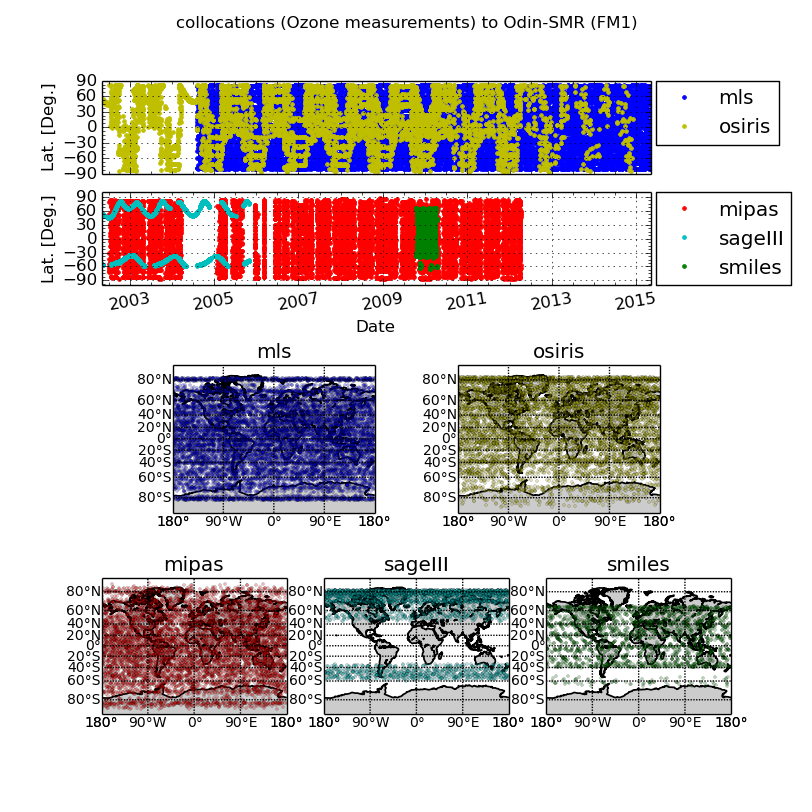
\includegraphics[width=17cm]{test_collocation_fm1.png}
\caption{VDS:Positions of collocated scans for frequency mode 1.}
\label{fig:vdsfm1}
\end{figure}


%The VDS consists of a selected subset of the \smr\ dataset, and correlative
%datasets to be used for validation purposes. 
The VDS should ideally include \smr\ measurements and correlative collocated 
data from the complete mission and for all geopraphical regions.
%The VDS can be seen as a dataset of \smr\ measurements and
%collocated measurements from the instrument described 
%in the preceeding section. 
In this section we describe how the VDS was constructed
in order to fulfill this criteria.

Two measurements are considered to be collocated if they
are close in time and space. The applied collocations
criteria are adjusted for the various sensors, in order
to result in a useful comparison dataset, as described below:

\smr\ and SMILES measurements are considered to be collocated if the 
differences in distance and observation time between the two profiles are
less than 300\,km and 1\,h, respectively.
All measurements that fulfill this criteria are included
in the VDS. This subset of the VDS
covers 60\degree\, N--40\degree\,S for the SMILES
active observation period, as can be seen in Fig.~\ref{fig:vdsfm1}.

\smr\ and SAGEIII measurements are considered to be collocated if the 
difference in distance and observation time between the two profiles are
less than 300\,km and and 3\,h, respectively.
This subset of the VDS covers approximately 80\degree\,N--50\degree\,N and
40\degree\,S--60\degree\,S for the SAGEIII active observation period, as can
be seen in Fig.~\ref{fig:vdsfm1}

A problem with a ``strict'' time difference criteria
between \smr\ and both ENVISAT/MIPAS and Aura/MLS
is that collocations are only found for high latitudes
 (around 80\degree\,N and around 80\degree\,S),
due to the fact each of these platform follows a sun-synchronous orbit
with quite different ascending equator crossing local times  
(18:00 hour for \smr\, 10:00 hour for ENVISAT/MIPAS,
 13:45 hour for Aura/MLS). 
Thus, for low latitudes the time difference criteria
is relaxed to 6\,hour for ENVISAT/MIPAS and Aura/MLS.
This gives effectively that collocated ENVISAT/MIPAS and Aura/MLS 
measurements can be found for almost all \smr\ measurements, and a strategy
to reduce the size of the VDS must be applied.

The set of collocated measurements for ENVISAT/MIPAS and Aura/MLS is reduced
in size in the following way:
For each \smr\ observation mode and month, five collocated scans each
for ENVISAT/MIPAS and Aura/MLS
are selected, within each 10\degree\ latitude bin
(85\degree\,N--75\degree\,N, 75\degree\,N--65\degree\,N, \ldots, 75\degree\,S--85\degree\,S),
to be included in the VDS. For the two outer latitude bins the
time difference criteria is 1\,h, while for the other bins it is set to 6\,h.
Figure~\ref{fig:vdsfm1} shows a graphical view of the position in
time and space for the measurements included in the VDS for
frequency mode 1 of \smr.   

The total number of measurements included in the VDS, for the various \smr\ frequency modes,
is displayed in Table~\ref{table:comp}. This gives that a few percent of the total \smr\
dataset is included in the VDS. Included measurements cover approximately 
all geographical positions and the complete observation period of \smr. 
